\documentclass[UTF8,a4paper,12pt]{ctexart}

\usepackage{amsmath}
\numberwithin{equation}{section}
\usepackage{amssymb}
\usepackage{bm}
\usepackage{graphicx}
\usepackage{float}
\usepackage{tikz}
\usetikzlibrary{arrows.meta,positioning}
\usepackage{fancyhdr}
\pagestyle{fancy}
\fancyhf{}
\fancyhead[R]{\thepage}
\renewcommand{\headrulewidth}{0pt}
\setlength{\headheight}{15pt}
\fancypagestyle{plain}{
	\fancyhf{}
	\fancyhead[R]{\thepage}
	\renewcommand{\headrulewidth}{0pt}
}

\renewcommand{\topfraction}{0.9}
\renewcommand{\bottomfraction}{0.7}
\renewcommand{\textfraction}{0.1}
\renewcommand{\floatpagefraction}{0.8}

\setlength{\abovedisplayskip}{6pt plus 2pt minus 3pt}
\setlength{\belowdisplayskip}{6pt plus 2pt minus 3pt}
\setlength{\abovedisplayshortskip}{3pt plus 1pt minus 2pt}
\setlength{\belowdisplayshortskip}{3pt plus 1pt minus 2pt}
\setlength{\textfloatsep}{8pt plus 2pt minus 2pt}
\setlength{\intextsep}{8pt plus 2pt minus 2pt}
\setlength{\abovecaptionskip}{4pt}

\usepackage[colorlinks=true,linkcolor=black,urlcolor=blue,citecolor=black]{hyperref}

\title{机器学习基础}
\date{\today}

\begin{document}

\maketitle

	在正式开始前，向大家介绍一本很好的学习教材————邱锡鹏老师所著的\href{https://nndl.ai/nndl-v2/}{《神经网络与深度学习》}。本文主要基于该教材的记录与笔记，并附上笔者自己的理解，如有错误或问题，欢迎指正与交流！

\section{概念}
	早在中学，我们就学过自变量和因变量。简单地说，由研究者主动操控的变量是自变量，随自变量变化而变化的量是因变量。因变量如何被自变量决定，取决于两者之间的映射关系。在初等数学中常见的映射关系有：一次函数 $y=kx+b$、二次函数 $y=ax^{2}+bx+c$、对数函数 $y=\ln x$以及各种初等函数及它们的线性组合。这些都是已知的、能写出具体表达式的映射关系。

	但生活中变量之间的关系，往往没有现成的表达式，也没有办法用已知的任何初等函数进行精确的表达，比如股市的走势如何变化，抛10次硬币出现正面朝上的次数是多少。于是人们想到近似的办法：做大量重复的实验，把结果一次次记录下来，再从中归纳规律。以抛硬币为例，前一百次里正面可能出现六七十次；抛到一万次，正面大约是五千多次；抛到十万次，正面所占的比例就越来越接近 $50\%$。

	值得思考的是：不管抛不抛、在实验次数越来越多的情况下，正面的占比似乎都趋向某个客观存在的值。它不会因为实验次数的多少而改变，只是随着实验次数增多，记录下来的正面出现的频率越来越接近于这个值。当然，我们知道在抛硬币现象中的正面出现占总实验次数的占比会随着实验次数的增加而收敛于$50\%$。虽然这件事在古典概率中早有记载，但仍为一个好的例子用来引出接下来的观点。正如大数定律所刻画的：设 $X_{1},X_{2},\ldots,X_{N}$ 是独立同分布的随机变量，期望 $\mathbb{E}[X_{i}]=\mu$，记样本均值 $\bar{X}_{N}=\frac{1}{N}\sum_{i=1}^{N}X_{i}$，则对任意 $\varepsilon>0$，
	\begin{equation}\label{eq:1.1}
	\lim_{N\to\infty}P\bigl(\bigl|\bar{X}_{N}-\mu\bigr|\ge\varepsilon\bigr)=0,
	\end{equation}
	即样本均值依概率收敛于真实期望。这里不妨把"依概率收敛"说清楚：对任意给定的正数 $\varepsilon$（无论多小），$\bar{X}_{N}$ 与真实期望 $\mu$ 的偏差超过 $\varepsilon$ 的概率，都随 $N$ 增大而趋于 $0$；换言之，只要实验次数足够多，$\bar{X}_{N}$ 几乎必然落在 $\mu$ 的任意小邻域内。
	
	古典概率模型中掷骰子是同样的例子：每次掷出的点数 $X_{i}$ 服从离散均匀分布，期望 $\mu=\frac{1+2+\cdots+6}{6}=3.5$，投掷次数足够多后，点数的平均值便稳定在 $3.5$ 附近，正如抛硬币时正面频率稳定在 $\frac{1}{2}$ 附近。也就是说，只要我们可以无限的做实验，再通过实验结论去反向推理，那么推理出来的模型就能无限逼近这个我们要找的客观存在于变量之间的映射规律。
	
	这种近似是非常完美的理论方法，这个思想的出现几乎是这一领域（映射关系）的一次革命，也就是说，凡是遇到复杂的变量关系问题，只需要极其粗暴的用这种近似的方法就能找出无限高精度的模型。可是新的解法出现了，新的问题当然也会随之出现。无限做实验的成本实在是太高了，在计算机发明以前，每次实验的时间成本是不可忽略的。即便是在之前的硬币实验中，抛一次硬币或许几秒或是十几秒就能结束，但真去抛一百万次、一亿次硬币，成本是惊人的。幸运的是，计算机最擅长的就是这种海量重复计算，一秒钟就能"抛"上几千万次。而机器学习正是利用了这一点：让计算机进行大规模的实验与计算，原来需要一个人花一辈子才能抛完的硬币，在今日或许只需要一分钟甚至一秒钟。机器学习这一领域也应运而生，核心其实很简单：训练出一个模型，使它能够根据输入预测输出，并且尽可能猜得准。

	在多数实际问题中，结果由若干因素共同决定——房价取决于面积、楼层、地段，明天是否降雨取决于温度、湿度、气压。将这些因素连同对应的结果记录下来，即构成一个样本，记作 $(\bm{x},y)$：$\bm{x}$ 是输入特征，$y$ 是标签，即模型需要预测的目标。

	因素只有一个时，输入是一个标量；因素有多个时，把它们拼在一起，输入就成了一个 $d$ 维向量：
	\begin{equation}\label{eq:1.2}
	\bm{x}^{(n)}
	=\left(x_1^{(n)},x_2^{(n)},\ldots,x_d^{(n)}\right)^{\mathsf{T}},
	\qquad n=1,2,\ldots,N,
	\end{equation}
	其中上标 $(n)$ 表示第 $n$ 个样本，$x_t^{(n)}$ 是它第 $t$ 维上的特征值。

	$N$ 个这样的样本合在一起就构成总数据集，这份总的数据集需要用于模型的训练、选择、评估。因此一般将其划分为三份（训练集、验证集、测试集）：训练集用于学习模型参数，模型从中总结规律；验证集用于选择超参数、判断何时停止训练；测试集仅在最后评估一次模型的真实水平，用于模拟未见过的新数据。
	
\begin{figure}[htbp]
	\centering
	\resizebox{0.88\textwidth}{!}{%
		\begin{tikzpicture}[
			>=Stealth,
			formula/.style={
				font=\small,
				align=center,
				inner sep=2pt
			},
			caption/.style={
				font=\small,
                align=center,
                text=black!75,
                inner sep=1pt
            },
            model/.style={
                rounded corners=12pt,
                draw=blue!55!black,
				fill=blue!8,
				line width=0.8pt,
				minimum width=2.6cm,
				minimum height=0.95cm,
				align=center,
				font=\small
			},
			arrow/.style={
				->,
				draw=gray!75,
				line width=0.9pt,
				shorten >=2pt,
				shorten <=2pt
			}
			]

			% 上方：推断 / 预测过程
			\node[formula] (input) at (-4.3,1.7) {$\bm{x}$};
			\node[model] (learned) at (0,1.7) {$f^{*}(\bm{x})$};
			\node[formula] (output) at (4.3,1.7)
			{$\hat{y}\ \text{或}\ \hat{p}(y\mid\bm{x})$};

        \node[caption,below=4pt of input] {输入};
        \node[caption,below=4pt of output] {输出};

        \draw[arrow] (input) -- (learned);
			\draw[arrow] (learned) -- (output);

			% 下方：学习 / 训练过程
			\node[formula] (dataset) at (-4.3,-1.2)
			{$\mathcal{D}=\left\{(\bm{x}^{(n)},y^{(n)})\right\}_{n=1}^{N}$};

			\node[model] (algorithm) at (0,-1.2) {$\mathcal{A}$};

			\node[formula] (functions) at (4.3,-1.2)
			{$\mathcal{F}=\left\{f_{1}(\bm{x}),f_{2}(\bm{x}),\ldots\right\}$};

        \node[caption,below=4pt of dataset] {训练样本集合};
        \node[caption,below=4pt of algorithm] {学习算法};
        \node[caption,below=4pt of functions] {函数集合};

        \draw[arrow] (dataset) -- (algorithm);
        \draw[arrow] (functions) -- (algorithm);
        \draw[arrow] (algorithm.north) -- (learned.south)
            node[midway,right=6pt,caption] {学习到的函数};

        \end{tikzpicture}%
    }
    \caption{机器学习基本流程示意图}
    \label{fig:ml_flow}
\end{figure}

	有了样本和数据集，接下来的问题是：模型从何而来、如何学习。图~\ref{fig:ml_flow} 概括了这一流程，从下到上读：学习之前需先划定搜索范围，即预设候选函数集合 $\mathcal{F}$（如所有一次函数，或某种结构固定、参数待定的所有神经网络）；学习算法 $\mathcal{A}$ 再根据训练集 $\mathcal{D}$，从 $\mathcal{F}$ 中选出最能拟合数据规律的函数，记为 $f^{*}$。

	学出的模型 $f^{*}(\bm{x})$ 接收新样本的输入 $\bm{x}$，输出预测 $\hat{y}$；概率问题中也可以输出条件概率 $\hat{p}(y\mid\bm{x})$。机器学习的核心，就是从训练样本中学会输入到输出的规律，并推广到没见过的数据。

\section{学习准则}

上一节给出了机器学习的整体流程。将这一流程落实，首先要明确以何种准则衡量模型的优劣：先在单个样本上定义损失函数，再在整体上给出风险最小化准则。

\subsection{损失函数}

监督学习通常假设样本 $(\bm{x},y)$ 是从一个未知但固定的分布 $p_r(\bm{x},y)$ 中独立抽取的。我们真正关心的是模型在真实分布上的平均损失，即期望风险：
\begin{equation}\label{eq:2.1}
\mathcal{R}(\bm{\theta})
=\mathbb{E}_{(\bm{x},y)\sim p_r(\bm{x},y)}
\bigl[\mathcal{L}\bigl(y,f(\bm{x};\bm{\theta})\bigr)\bigr],
\end{equation}
其中 $\mathcal{L}(\cdot,\cdot)$ 为损失函数。$p_r$ 未知，期望风险算不出来，只能先选好损失函数，再用训练数据近似优化。

\noindent\textbf{0-1 损失函数} 最直观的损失就是错误率：
\begin{equation}\label{eq:2.2}
\mathcal{L}\bigl(y,f(\bm{x};\bm{\theta})\bigr)
=\mathbb{I}\bigl(y\neq f(\bm{x};\bm{\theta})\bigr),
\end{equation}
其中 $\mathbb{I}(\cdot)$ 为指示函数：预测错误时取 $1$，否则取 $0$。它不连续、导数几乎处处为 $0$，无法用梯度方法优化，实践中常用连续可微的损失替代。

\noindent\textbf{平方损失函数} 用于标签为实值的回归任务，一般不适用于分类：
\begin{equation}\label{eq:2.3}
\mathcal{L}\bigl(y,f(\bm{x};\bm{\theta})\bigr)
=\frac{1}{2}\bigl(y-f(\bm{x};\bm{\theta})\bigr)^{2}.
\end{equation}

\noindent\textbf{交叉熵损失函数} 用于分类问题。设标签 $y\in\{1,\ldots,C\}$，模型输出 $f(\bm{x};\bm{\theta})\in[0,1]^{C}$ 为各类别的预测概率，总和为 $1$；标签写成 one-hot 向量 $\bm{y}$（真实类别那一维为 $1$，其余为 $0$），它本身就是标签的真实分布。

两个分布 $p$、$q$ 之间的交叉熵定义为
\begin{equation}\label{eq:2.4}
H(p,q)=-\sum_{x}p(x)\log q(x),
\end{equation}
可以这样理解：要压缩服从 $p$ 的数据，最优编码会给常见符号配短码、罕见符号配长码，符号 $x$ 的码长约为 $-\log p(x)$，此时平均码长最小。若错按 $q$ 设计编码，码长变成 $-\log q(x)$，而符号出现的频率仍由 $p$ 决定，平均码长就成了交叉熵 $H(p,q)$。注意它不对称：$H(p,q)$ 按 $p$ 取期望，$H(q,p)$ 按 $q$ 取期望，二者一般不相等。分类任务中真实分布必须放在前面：我们关心的是"数据来自 $p$，用模型给出的 $q$ 去刻画它要付多大代价"；而且 $p(x)=0$ 的项在 $H(p,q)$ 中恒为 $0$，一旦交换位置，这些项的影响就完全不同了。

交叉熵可以分解为
\begin{equation}\label{eq:2.5}
H(p,q)=H(p)+D_{\mathrm{KL}}(p\|q),
\end{equation}
其中 $H(p)=-\sum_{x}p(x)\log p(x)$ 是 $p$ 的熵，即用最优编码压缩 $p$ 所需的最少平均信息量，是压缩的下限；第二项
\begin{equation}\label{eq:2.6}
D_{\mathrm{KL}}(p\|q)=\sum_{x}p(x)\log\frac{p(x)}{q(x)}
\end{equation}
是 KL 散度，即错用 $q$ 编码比最优编码多付出的平均信息量超出越多，$q$ 与 $p$ 的差异越大。它有两个关键性质。

一是非负：由不等式 $\log x\le x-1$，
\begin{equation}\label{eq:2.7}
\begin{aligned}
-D_{\mathrm{KL}}(p\|q)
&=\sum_{x}p(x)\log\frac{q(x)}{p(x)}
\le\sum_{x}p(x)\Bigl(\frac{q(x)}{p(x)}-1\Bigr)\\
&=\sum_{x}q(x)-\sum_{x}p(x)=0,
\end{aligned}
\end{equation}
等号仅当 $p$、$q$ 几乎处处相同时成立。所以交叉熵永远不小于熵，$q=p$ 时取到下界。

二是不对称：$D_{\mathrm{KL}}(p\|q)\ne D_{\mathrm{KL}}(q\|p)$。原因在权重：对数按 $p$ 加权，$p$ 概率大的地方 $q$ 必须同样大，否则 $\log\frac{p(x)}{q(x)}$ 会非常大；而 $q$ 有、$p$ 没有的项不参与求和，不产生任何惩罚。因此它着重惩罚"真实常见却预测罕见"的情形，而不惩罚"预测多余"，故并非严格意义上的距离。

熵 $H(p)$ 由数据本身决定，与参数无关，所以最小化交叉熵等价于最小化 KL 散度，即让预测分布尽量贴近真实分布。这就是分类问题用交叉熵损失的统计学解释。

代入 one-hot 标签，交叉熵损失简化为
\begin{equation}\label{eq:2.8}
\mathcal{L}\bigl(\bm{y},f(\bm{x};\bm{\theta})\bigr)
=-\bm{y}^{\mathsf{T}}\log f(\bm{x};\bm{\theta})
=-\log f_y(\bm{x};\bm{\theta}),
\end{equation}
即真实类别预测概率的负对数。由于 $f_y(\bm{x};\bm{\theta})$ 正是真实类别的似然，交叉熵损失也就是负对数似然，最小化它等价于极大似然估计。

\noindent\textbf{Hinge 损失函数} 用于二分类。取 $y\in\{-1,+1\}$，模型输出实数 $f(\bm{x};\bm{\theta})$，定义为
\begin{equation}\label{eq:2.9}
\mathcal{L}\bigl(y,f(\bm{x};\bm{\theta})\bigr)
=\max\bigl(0,\,1-yf(\bm{x};\bm{\theta})\bigr)
\triangleq\bigl[1-yf(\bm{x};\bm{\theta})\bigr]_{+}.
\end{equation}
为什么这样设计？预测正确的充要条件是 $yf(\bm{x};\bm{\theta})>0$，但最理想的 0-1 损失不可导。Hinge 损失是它的分段线性凸上界，并且更进一步：要求 $yf(\bm{x};\bm{\theta})\ge 1$ 才零惩罚，即不仅要分对，还需留出至少为 $1$ 的间隔。这样设计有两个好处：它是凸函数，便于优化，且与支持向量机最大间隔的思想一致；外层的 $\max(0,\cdot)$ 使分类正确且间隔充足的样本不产生梯度，仅间隔不足或分类错误的样本推动参数更新。

\subsection{风险最小化准则}

三种"风险"的关系是学习准则的核心。期望风险是真正的目标，但算不出来；手头只有训练集，于是用训练集上的平均损失来近似，即经验风险：
\begin{equation}\label{eq:2.10}
\mathcal{R}^{\mathrm{emp}}(\bm{\theta})
=\frac{1}{N}\sum_{n=1}^{N}
\mathcal{L}\bigl(y^{(n)},f(\bm{x}^{(n)};\bm{\theta})\bigr).
\end{equation}
由大数定律，$N\to\infty$ 时经验风险收敛到期望风险；但样本总是有限的，经验风险小不代表期望风险小，两者之差就是泛化误差。经验风险最小化准则
\begin{equation}\label{eq:2.11}
\bm{\theta}^{*}=\arg\min_{\bm{\theta}}\ \mathcal{R}^{\mathrm{emp}}(\bm{\theta})
\end{equation}
只关注训练误差：模型过于复杂时，会将噪声也当作规律学习，导致过拟合；反之，模型能力不足、连训练数据都拟合不佳时，则为欠拟合。图~\ref{fig:fit} 给出了这三种情形的直观对比。

\begin{figure}[htbp]
	\centering
	\begin{minipage}{0.3\textwidth}
		\centering
		\begin{tikzpicture}[scale=0.6]
			\draw[->,gray!70] (0,0) -- (5.9,0);
			\draw[->,gray!70] (0,0) -- (0,5.9);
			\foreach \x/\y in {0.3/0.7,0.8/1.3,1.3/1.5,1.8/2.3,2.3/2.2,2.8/3.3,3.3/3.1,3.8/4.2,4.3/4.3,4.8/5.2,5.3/5.4}
				\fill[blue!60!black] (\x,\y) circle (1.6pt);
			\draw[red!70!black,line width=0.9pt] (0,0.9) -- (5.6,5.0);
		\end{tikzpicture}\\[2pt]
		{\small 欠拟合}
	\end{minipage}\hfill
	\begin{minipage}{0.3\textwidth}
		\centering
		\begin{tikzpicture}[scale=0.6]
			\draw[->,gray!70] (0,0) -- (5.9,0);
			\draw[->,gray!70] (0,0) -- (0,5.9);
			\foreach \x/\y in {0.3/0.7,0.8/1.3,1.3/1.5,1.8/2.3,2.3/2.2,2.8/3.3,3.3/3.1,3.8/4.2,4.3/4.3,4.8/5.2,5.3/5.4}
				\fill[blue!60!black] (\x,\y) circle (1.6pt);
			\draw[red!70!black,line width=0.9pt] plot[smooth] coordinates
				{(0,0.5)(0.7,0.9)(1.5,1.6)(2.3,2.5)(3.1,3.4)(3.9,4.3)(4.7,5.0)(5.4,5.5)};
		\end{tikzpicture}\\[2pt]
		{\small 正常}
	\end{minipage}\hfill
	\begin{minipage}{0.3\textwidth}
		\centering
		\begin{tikzpicture}[scale=0.6]
			\draw[->,gray!70] (0,0) -- (5.9,0);
			\draw[->,gray!70] (0,0) -- (0,5.9);
			\foreach \x/\y in {0.3/0.7,0.8/1.3,1.3/1.5,1.8/2.3,2.3/2.2,2.8/3.3,3.3/3.1,3.8/4.2,4.3/4.3,4.8/5.2,5.3/5.4}
				\fill[blue!60!black] (\x,\y) circle (1.6pt);
			\draw[red!70!black,line width=0.9pt] plot[smooth,tension=1.1] coordinates
				{(0,0.7)(0.3,0.7)(0.8,1.3)(1.3,1.5)(1.8,2.3)(2.3,2.2)(2.8,3.3)(3.3,3.1)(3.8,4.2)(4.3,4.3)(4.8,5.2)(5.3,5.4)};
		\end{tikzpicture}\\[2pt]
		{\small 过拟合}
	\end{minipage}
	\caption{欠拟合、正常与过拟合的直观对比}
	\label{fig:fit}
\end{figure}

结构风险最小化在经验风险后面加一个复杂度惩罚项：
\begin{equation}\label{eq:2.12}
\bm{\theta}^{*}
=\arg\min_{\bm{\theta}}\ \mathcal{R}^{\mathrm{emp}}(\bm{\theta})
+\lambda\,\Omega(\bm{\theta}),
\end{equation}
其中 $\Omega(\bm{\theta})$ 衡量模型复杂度，$\lambda\ge 0$ 为权衡系数。理论上，期望风险大致以"经验风险加复杂度项"为上界，所以最小化结构风险就是在压低这个上界，比单看经验风险更接近真正的目标。最常用 $\ell_2$ 正则化；$\ell_1$ 会带来稀疏解。从贝叶斯角度看，正则化就是给参数加先验。

综上：期望风险是目标，经验风险是有限样本下的近似，结构风险则在近似之上再施加一项复杂度约束。$\lambda$ 这类超参数靠验证集挑选；数据少时用 $K$ 折交叉验证：把数据均分 $K$ 份，轮流用一份验证、其余训练，取 $K$ 次结果的平均。

\section{偏差-方差分解}

上一节提到，模型太简单会欠拟合，太复杂会过拟合。偏差-方差分解把这件事定量地拆开来看。以回归问题、平方损失为例（结论同样适用于分类），模型的期望风险为
\begin{equation}\label{eq:3.1}
\mathcal{R}(f)
=\mathbb{E}_{(\bm{x},y)\sim p_r(\bm{x},y)}\bigl[\bigl(y-f(\bm{x})\bigr)^{2}\bigr].
\end{equation}
给定 $\bm{x}$，真实分布下的 $y$ 是随机变量，围绕一个理论均值波动，这个理论均值记为
\begin{equation}\label{eq:3.2}
f^{*}(\bm{x})=\mathbb{E}_{y\sim p_r(y\mid\bm{x})}[y],
\end{equation}
它代表数据背后的真实规律；$y$ 对 $f^{*}(\bm{x})$ 的偏离就是噪声，噪声的均值为 $0$。

在 $f^{*}$ 处把期望风险拆开。约定 $\mathbb{E}_{\bm{x},y}$ 对 $(\bm{x},y)\sim p_r(\bm{x},y)$ 取期望，$\mathbb{E}_{y\mid\bm{x}}$ 固定 $\bm{x}$、只对 $y$ 取期望：
\begin{equation}\label{eq:3.3}
\begin{aligned}
\mathcal{R}(f)
&=\mathbb{E}_{\bm{x},y}\Bigl[\bigl(y-f^{*}(\bm{x})+f^{*}(\bm{x})-f(\bm{x})\bigr)^{2}\Bigr]\\
&=\mathbb{E}_{\bm{x},y}\bigl[\bigl(y-f^{*}(\bm{x})\bigr)^{2}\bigr]
+\mathbb{E}_{\bm{x}}\bigl[\bigl(f(\bm{x})-f^{*}(\bm{x})\bigr)^{2}\bigr]\\
&\qquad+2\,\mathbb{E}_{\bm{x},y}\bigl[\bigl(y-f^{*}(\bm{x})\bigr)\bigl(f^{*}(\bm{x})-f(\bm{x})\bigr)\bigr].
\end{aligned}
\end{equation}
交叉项为 $0$，用全期望公式把期望拆成"先固定 $\bm{x}$ 对 $y$ 取、再对 $\bm{x}$ 取"即可看出：
\begin{equation}\label{eq:3.4}
\begin{aligned}
&\mathbb{E}_{\bm{x},y}\bigl[\bigl(y-f^{*}(\bm{x})\bigr)\bigl(f^{*}(\bm{x})-f(\bm{x})\bigr)\bigr]\\
&=\mathbb{E}_{\bm{x}}\Bigl[\mathbb{E}_{y\mid\bm{x}}\bigl[\bigl(y-f^{*}(\bm{x})\bigr)\bigl(f^{*}(\bm{x})-f(\bm{x})\bigr)\bigr]\Bigr]\\
&=\mathbb{E}_{\bm{x}}\Bigl[\bigl(f^{*}(\bm{x})-f(\bm{x})\bigr)\,\mathbb{E}_{y\mid\bm{x}}\bigl[y-f^{*}(\bm{x})\bigr]\Bigr]=0.
\end{aligned}
\end{equation}
固定 $\bm{x}$ 后 $f^{*}(\bm{x})-f(\bm{x})$ 是常数，可提出 $\mathbb{E}_{y\mid\bm{x}}$；而 $\mathbb{E}_{y\mid\bm{x}}[y-f^{*}(\bm{x})]=0$给定 $\bm{x}$ 时真实值 $y$ 都围绕 $f^{*}(\bm{x})$ 波动，即噪声均值为 $0$。于是
\begin{equation}\label{eq:3.5}
\mathcal{R}(f)
=\mathbb{E}_{\bm{x}}\bigl[\bigl(f(\bm{x})-f^{*}(\bm{x})\bigr)^{2}\bigr]+\varepsilon,
\qquad
\varepsilon=\mathbb{E}_{\bm{x},y}\bigl[\bigl(y-f^{*}(\bm{x})\bigr)^{2}\bigr].
\end{equation}
$\varepsilon$ 是噪声的期望大小，与 $f$ 无关，理论最优模型也避免不了；第一项是 $f$ 与 $f^{*}$ 的差距，才是能优化的部分。故 $\mathcal{R}(f)$ 在 $f=f^{*}$ 处取最小，$f^{*}$ 即平方损失下的理论最优模型。

但 $f(\bm{x})$ 在具体训练集 $\mathcal{D}$ 上学出，更换训练数据便得到不同的模型。评价学习算法本身，需对训练集取平均。记 $f_{\mathcal{D}}$ 为在 $\mathcal{D}$ 上学到的模型，对单个 $\bm{x}$ 插入中间项 $\mathbb{E}_{\mathcal{D}}[f_{\mathcal{D}}(\bm{x})]$ 后展开：
\begin{equation}\label{eq:3.6}
\begin{aligned}
&\mathbb{E}_{\mathcal{D}}\bigl[\bigl(f_{\mathcal{D}}(\bm{x})-f^{*}(\bm{x})\bigr)^{2}\bigr]\\
&=\mathbb{E}_{\mathcal{D}}\Bigl[\bigl(f_{\mathcal{D}}(\bm{x})-\mathbb{E}_{\mathcal{D}}[f_{\mathcal{D}}(\bm{x})]
+\mathbb{E}_{\mathcal{D}}[f_{\mathcal{D}}(\bm{x})]-f^{*}(\bm{x})\bigr)^{2}\Bigr]\\
&=\underbrace{\bigl(\mathbb{E}_{\mathcal{D}}[f_{\mathcal{D}}(\bm{x})]-f^{*}(\bm{x})\bigr)^{2}}_{\text{偏差}^{2}}
+\underbrace{\mathbb{E}_{\mathcal{D}}\Bigl[\bigl(f_{\mathcal{D}}(\bm{x})-\mathbb{E}_{\mathcal{D}}[f_{\mathcal{D}}(\bm{x})]\bigr)^{2}\Bigr]}_{\text{方差}},
\end{aligned}
\end{equation}
这里的交叉项同样为 $0$：记平均模型 $\bar{f}(\bm{x})=\mathbb{E}_{\mathcal{D}}[f_{\mathcal{D}}(\bm{x})]$，固定 $\bm{x}$ 时 $\bar{f}(\bm{x})$、$f^{*}(\bm{x})$ 都与 $\mathcal{D}$ 无关，是常数，第二个因子可提出期望：
\begin{equation}\label{eq:3.7}
\begin{aligned}
&\mathbb{E}_{\mathcal{D}}\Bigl[\bigl(f_{\mathcal{D}}(\bm{x})-\bar{f}(\bm{x})\bigr)
\bigl(\bar{f}(\bm{x})-f^{*}(\bm{x})\bigr)\Bigr]\\
&=\bigl(\bar{f}(\bm{x})-f^{*}(\bm{x})\bigr)\,
\mathbb{E}_{\mathcal{D}}\bigl[f_{\mathcal{D}}(\bm{x})-\bar{f}(\bm{x})\bigr]=0,
\end{aligned}
\end{equation}
因为 $\mathbb{E}_{\mathcal{D}}[f_{\mathcal{D}}(\bm{x})-\bar{f}(\bm{x})]=\bar{f}(\bm{x})-\bar{f}(\bm{x})=0$。代回上式，得最终分解：
\begin{equation}\label{eq:3.8}
\mathcal{R}(f)=\text{偏差}^{2}+\text{方差}+\varepsilon.
\end{equation}

图~\ref{fig:bv_targets} 用打靶比喻四种组合：靶心是最优模型 $f^{*}(\bm{x})$，蓝点是不同训练集上学到的 $f_{\mathcal{D}}(\bm{x})$；点群中心离靶心的距离是偏差，点群散开的程度是方差。

\begin{figure}[htbp]
	\centering
	\begin{minipage}{0.23\textwidth}
		\centering
		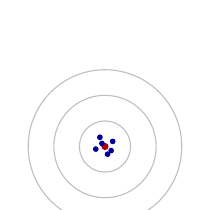
\begin{tikzpicture}[scale=0.65]
			\draw[gray!50] (0,0) circle (0.5);
			\draw[gray!50] (0,0) circle (1.0);
			\draw[gray!50] (0,0) circle (1.5);
			\fill[red!70!black] (0,0) circle (2pt);
			\foreach \x/\y in {0.15/0.1,-0.1/0.18,0.05/-0.15,-0.18/-0.05,0.12/-0.08,-0.06/0.06}
				\fill[blue!60!black] (\x,\y) circle (1.6pt);
		\end{tikzpicture}\\[2pt]
		{\small 低偏差、低方差}
	\end{minipage}\hfill
	\begin{minipage}{0.23\textwidth}
		\centering
		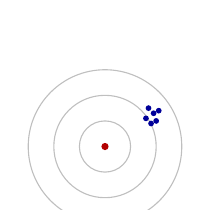
\begin{tikzpicture}[scale=0.65]
			\draw[gray!50] (0,0) circle (0.5);
			\draw[gray!50] (0,0) circle (1.0);
			\draw[gray!50] (0,0) circle (1.5);
			\fill[red!70!black] (0,0) circle (2pt);
			\foreach \x/\y in {0.95/0.65,0.8/0.55,1.0/0.5,0.85/0.75,0.9/0.45,1.05/0.7}
				\fill[blue!60!black] (\x,\y) circle (1.6pt);
		\end{tikzpicture}\\[2pt]
		{\small 高偏差、低方差}
	\end{minipage}\hfill
	\begin{minipage}{0.23\textwidth}
		\centering
		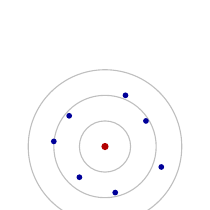
\begin{tikzpicture}[scale=0.65]
			\draw[gray!50] (0,0) circle (0.5);
			\draw[gray!50] (0,0) circle (1.0);
			\draw[gray!50] (0,0) circle (1.5);
			\fill[red!70!black] (0,0) circle (2pt);
			\foreach \x/\y in {0.8/0.5,-0.7/0.6,0.2/-0.9,-0.5/-0.6,1.1/-0.4,-1.0/0.1,0.4/1.0}
				\fill[blue!60!black] (\x,\y) circle (1.6pt);
		\end{tikzpicture}\\[2pt]
		{\small 低偏差、高方差}
	\end{minipage}\hfill
	\begin{minipage}{0.23\textwidth}
		\centering
		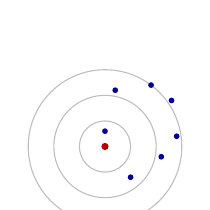
\begin{tikzpicture}[scale=0.65]
			\draw[gray!50] (0,0) circle (0.5);
			\draw[gray!50] (0,0) circle (1.0);
			\draw[gray!50] (0,0) circle (1.5);
			\fill[red!70!black] (0,0) circle (2pt);
			\foreach \x/\y in {1.3/0.9,0.2/1.1,1.1/-0.2,0.0/0.3,1.4/0.2,0.5/-0.6,0.9/1.2}
				\fill[blue!60!black] (\x,\y) circle (1.6pt);
		\end{tikzpicture}\\[2pt]
		{\small 高偏差、高方差}
	\end{minipage}
	\caption{偏差与方差的四种组合}
	\label{fig:bv_targets}
\end{figure}

偏差是平均模型与最优模型的差距，衡量拟合能力；方差是模型随训练集变动的程度，衡量对数据扰动的敏感度。两者此消彼长：复杂度升高，偏差减小、方差增大，于是过拟合。增大正则化系数 $\lambda$ 可抑制方差，但偏差随之上升，$\lambda$ 过大时期望风险反而回升；方差还会随样本增多而减小，数据充足时便可采用拟合能力更强的模型以降低偏差。注意最优复杂度并不一定落在偏差曲线与方差曲线的交点。

\begin{figure}[H]
	\centering
	\begin{tikzpicture}[x=1.4cm,y=0.68cm]
		\draw[->,gray!70] (0,0) -- (6.4,0);
		\draw[->,gray!70] (0,0) -- (0,5.1);
		\node[below left=2pt] at (6.4,0) {模型复杂度};
		\node[left] at (0,5.05) {期望风险};
		% 偏差^2
		\draw[blue!70!black,line width=1pt] plot[smooth] coordinates
			{(0.5,3.2)(1.5,2.0)(2.5,1.3)(3.5,0.85)(4.5,0.55)(5.5,0.4)};
		% 方差
		\draw[red!70!black,line width=1pt] plot[smooth] coordinates
			{(0.5,0.2)(1.5,0.5)(2.5,1.0)(3.5,1.7)(4.5,2.6)(5.5,3.6)};
		% 期望风险 = 偏差^2 + 方差 + 噪声
		\draw[line width=1.2pt] plot[smooth] coordinates
			{(0.5,3.7)(1.5,2.8)(2.5,2.6)(3.5,2.85)(4.5,3.45)(5.5,4.3)};
		% 噪声水平
		\draw[dashed,gray] (0,0.3) -- (5.8,0.3)
			node[above,font=\small,text=black] {$\varepsilon$};
		% 最优复杂度
		\draw[dashed,red!70!black] (2.7,0) -- (2.7,4.4);
		\node[below,font=\small] at (2.7,0) {最优复杂度};
		% 图例
		\draw[blue!70!black,line width=1pt] (0.3,4.7) -- (0.9,4.7)
			node[right,font=\small,text=black] {偏差$^{2}$};
		\draw[red!70!black,line width=1pt] (2.35,4.7) -- (2.95,4.7)
			node[right,font=\small,text=black] {方差};
		\draw[line width=1.2pt] (4.15,4.7) -- (4.75,4.7)
			node[right,font=\small,text=black] {期望风险};
	\end{tikzpicture}
	\caption{期望风险、偏差与方差随模型复杂度的变化}
	\label{fig:bv_tradeoff}
\end{figure}

\section{优化算法}

学习准则确定了优化目标，接下来的问题是如何求解最优参数。先分清两个概念：模型参数 $\bm{\theta}$ 由优化算法直接学习；学习率、正则化系数、网络层数这类决定模型结构或优化策略的量叫超参数，无法从训练中学得，通常靠人工经验、网格搜索、随机搜索等方法结合验证集来选。

最常用的优化算法是梯度下降：梯度指向增长最快的方向，沿负梯度走下降最快。第 $t$ 次迭代的更新公式~\eqref{eq:4.1} 为
\begin{equation}\label{eq:4.1}
\bm{\theta}_{t+1}
=\bm{\theta}_{t}-\alpha\,\frac{\partial\mathcal{R}(\bm{\theta})}{\partial\bm{\theta}_{t}}
=\bm{\theta}_{t}-\alpha\cdot\frac{1}{N}\sum_{n=1}^{N}
\frac{\partial\mathcal{L}\bigl(y^{(n)},f(\bm{x}^{(n)};\bm{\theta})\bigr)}{\partial\bm{\theta}},
\end{equation}
其中 $\alpha$ 为学习率。

按每次迭代用多少样本，梯度下降分三种。记单个样本的梯度为
\begin{equation}\label{eq:4.2}
\bm{g}^{(n)}(\bm{\theta})
=\frac{\partial\mathcal{L}\bigl(y^{(n)},f(\bm{x}^{(n)};\bm{\theta})\bigr)}{\partial\bm{\theta}},
\end{equation}
三者的区别在于更新用的梯度怎么算：

批量梯度下降用全体样本的平均梯度，
\begin{equation}\label{eq:4.3}
\bm{\theta}_{t+1}
=\bm{\theta}_{t}-\alpha\cdot\frac{1}{N}\sum_{n=1}^{N}\bm{g}^{(n)}(\bm{\theta}_{t}),
\end{equation}
每步方向准确，但计算一次梯度需遍历整个训练集，数据量大时开销过高。

随机梯度下降每次随机取一个样本，直接用它的梯度更新：
\begin{equation}\label{eq:4.4}
\bm{\theta}_{t+1}=\bm{\theta}_{t}-\alpha\,\bm{g}^{(n)}(\bm{\theta}_{t}).
\end{equation}
单步计算量极小。其可行性在于：单样本梯度是全样本梯度的无偏估计随机抽取一个样本时 $\mathbb{E}_{n}\bigl[\bm{g}^{(n)}\bigr]=\frac{1}{N}\sum_{n=1}^{N}\bm{g}^{(n)}$，单次方向虽有偏差，平均而言却与全样本梯度一致，从长期看更新方向正确；单样本带来的噪声甚至有助于跳出非凸问题中较差的局部区域。其缺点是无法并行：每次只处理一个样本，$N$ 次更新只能串行进行，无法组织成矩阵批量运算，也就无法利用 GPU 的并行能力。

小批量梯度下降每次随机取 $K$ 个样本组成子集 $\mathcal{S}_{t}$，用它们的平均梯度更新：
\begin{equation}\label{eq:4.5}
\bm{\theta}_{t+1}
=\bm{\theta}_{t}-\alpha\cdot\frac{1}{K}\sum_{(\bm{x}^{(n)},y^{(n)})\in\mathcal{S}_{t}}\bm{g}^{(n)}(\bm{\theta}_{t}),
\end{equation}
$K$ 实践中常取 $2$ 的幂。它是前两种的折中：平均 $K$ 个样本后梯度噪声比随机梯度小，同时一个批次的计算可以组织成矩阵运算并行完成，兼顾效率与稳定，是深度学习的主流做法。

另外还可以用提前停止缓解过拟合（图~\ref{fig:earlystop}）：训练误差持续下降、验证误差却开始回升时，就终止训练。

\begin{figure}[tbp]
	\centering
	\begin{tikzpicture}[x=1.5cm,y=1.1cm]
		\draw[->,gray!70] (0,0) -- (6.6,0);
		\draw[->,gray!70] (0,0) -- (0,3.3);
		\node[below] at (6.5,0) {迭代次数};
		\node[left] at (0,3.25) {错误率};
		% 训练集误差
		\draw[blue!70!black,line width=1pt] plot[smooth] coordinates
			{(0,2.6)(1,1.7)(2,1.15)(3,0.8)(4,0.55)(5,0.4)(6,0.28)};
		% 验证集误差
		\draw[red!70!black,line width=1pt] plot[smooth] coordinates
			{(0,2.7)(1,2.0)(2,1.5)(2.8,1.28)(3.5,1.35)(4.3,1.6)(5,1.95)(6,2.35)};
		\draw[dashed,gray] (2.8,0) -- (2.8,2.95);
		\node[above,font=\small] at (2.8,2.95) {提前停止};
		\node[font=\small,text=black!70] at (5.1,1.0) {过拟合区域};
		% 图例
		\draw[blue!70!black,line width=1pt] (4.1,2.95) -- (4.75,2.95)
			node[right,font=\small,text=black] {训练集};
		\draw[red!70!black,line width=1pt] (4.1,2.4) -- (4.75,2.4)
			node[right,font=\small,text=black] {验证集};
	\end{tikzpicture}
	\caption{提前停止示意图}
	\label{fig:earlystop}
\end{figure}

\section{评价指标}

模型训练完成后，还需一套指标在测试集上评价其表现。分类问题最常用的指标是准确率和错误率：
\begin{equation}\label{eq:5.1}
\mathcal{A}=\frac{1}{N'}\sum_{n=1}^{N'}\mathbb{I}\bigl(y^{(n)}=\hat{y}^{(n)}\bigr),
\qquad
\mathcal{E}=1-\mathcal{A}.
\end{equation}

准确率是所有类别的整体平均。要看单个类别的表现，对类别 $c$ 把预测结果分四种：真正例 $\mathrm{TP}_c$（真实为 $c$，预测也为 $c$）、假负例 $\mathrm{FN}_c$（真实为 $c$，预测非 $c$）、假正例 $\mathrm{FP}_c$（真实非 $c$，预测为 $c$）、真负例 $\mathrm{TN}_c$（真实非 $c$，预测也非 $c$），整理成混淆矩阵，如图~\ref{fig:confusion} 所示。

\begin{figure}[htbp]
	\centering
	\begin{tikzpicture}[font=\small]
		\draw (0,0) rectangle (4.4,3.0);
		\draw (2.2,0) -- (2.2,3.0);
		\draw (0,1.5) -- (4.4,1.5);
		\node at (1.1,2.25) {$\mathrm{TP}_c$};
		\node at (3.3,2.25) {$\mathrm{FN}_c$};
		\node at (1.1,0.75) {$\mathrm{FP}_c$};
		\node at (3.3,0.75) {$\mathrm{TN}_c$};
		\node[above] at (1.1,3.0) {$\hat{y}=c$};
		\node[above] at (3.3,3.0) {$\hat{y}\neq c$};
		\node[above=16pt] at (2.2,3.0) {预测类别};
		\node[left] at (0,2.25) {$y=c$};
		\node[left] at (0,0.75) {$y\neq c$};
		\node[rotate=90] at (-1.75,1.5) {真实类别};
	\end{tikzpicture}
	\caption{类别 $c$ 的混淆矩阵}
	\label{fig:confusion}
\end{figure}

精确率是"预测为 $c$ 的样本中有多少是真的"，召回率是"真实为 $c$ 的样本中找回了多少"：
\begin{equation}\label{eq:5.2}
\mathcal{P}_c=\frac{\mathrm{TP}_c}{\mathrm{TP}_c+\mathrm{FP}_c},
\qquad
\mathcal{R}_c=\frac{\mathrm{TP}_c}{\mathrm{TP}_c+\mathrm{FN}_c}.
\end{equation}
两者往往此消彼长，常用调和平均 $F$ 值综合（$\beta=1$ 时即 F1 值）：
\begin{equation}\label{eq:5.3}
\mathcal{F}_c
=\frac{(1+\beta^{2})\times\mathcal{P}_c\times\mathcal{R}_c}
{\beta^{2}\times\mathcal{P}_c+\mathcal{R}_c}.
\end{equation}

汇总所有类别有两种平均方式：宏平均先算各类指标再取平均，各类别权重相同；微平均先汇总各类的 $\mathrm{TP}$、$\mathrm{FP}$、$\mathrm{FN}$ 再算，易被大类别主导，故类别不均衡时宏平均更能反映小类性能。调整分类阈值还可画出 ROC、PR 曲线，以 AUC 作更全面的评价。最后一个易忽视的维度是概率校准：模型给出 $0.9$ 的预测概率，这些预测中就该有约九成正确，否则概率输出不可信。



\end{document}
